% Sample file on how to use subfiles.
\documentclass[ExampleMasters.tex]{subfiles}

\begin{document}
\clearpage
\chapter{Steering Model}
\label{chap:steering_model}

\section{Rapid Control Prototyping}
\label{sec:rapid_proto}

In automotive software development standardized processes are applied to assure structured work. The V-model which derives its name from the characteristic shape constitutes one graphic representations of the sequence of steps towards the finished overall system. It also gives an approximate impression about the level of detail of each of the steps on the vertical axle, as well as chronological progress on the horizontal. A simplified version of this V-model can be seen in figure \ref{fig:v_model}. First the user or customer needs are analyzed and put into a schematic formulation of the system showing the logic dependencies and underlying physical working principles. This is usually done in a semi-standardized fashion utilizing Unified Markup Language (UML) or similiar diagrams, preventing non-specific prose to ensure less room for mis-communication and better readability. Technical decisions and limitations are not yet considered. After the logical system and dependencies have been established they will be analyzed and broken down to actual technical system descriptions defining also which subsystem will take over which function, what parts are to be realised as software or hardware (e.g. filtering, safety functions). The different parts of the technical system are then specified in detail, defining interfaces between different software sub-system, operational states and distribution of functions over sub-systems. The fourth step will define the specifications for the software in details for example: data types, control sequences, decision structures, real-time behaviour. Finally the actual design step will implement these specification with regards to the hardware limitations (RAM/ROM, processing power), computation methods, data handling (detailed format, variable types, utilization of parameters or variables). To compile the system from the component-level sub-system a similar hierachy is used in inverse. The corresponding steps of the project definition and specification phase (left side of the schematic) are supposed to provide test-procedures and goals. If necessary after insufficient test outcomes, another iteration of the previous step will be performed (vertical iterations). A similar sequence of development steps is applied to develop the hardware platform in parallel.\cite{automotive_software_engineering}

\begin{figure*}[htpb]
\centering
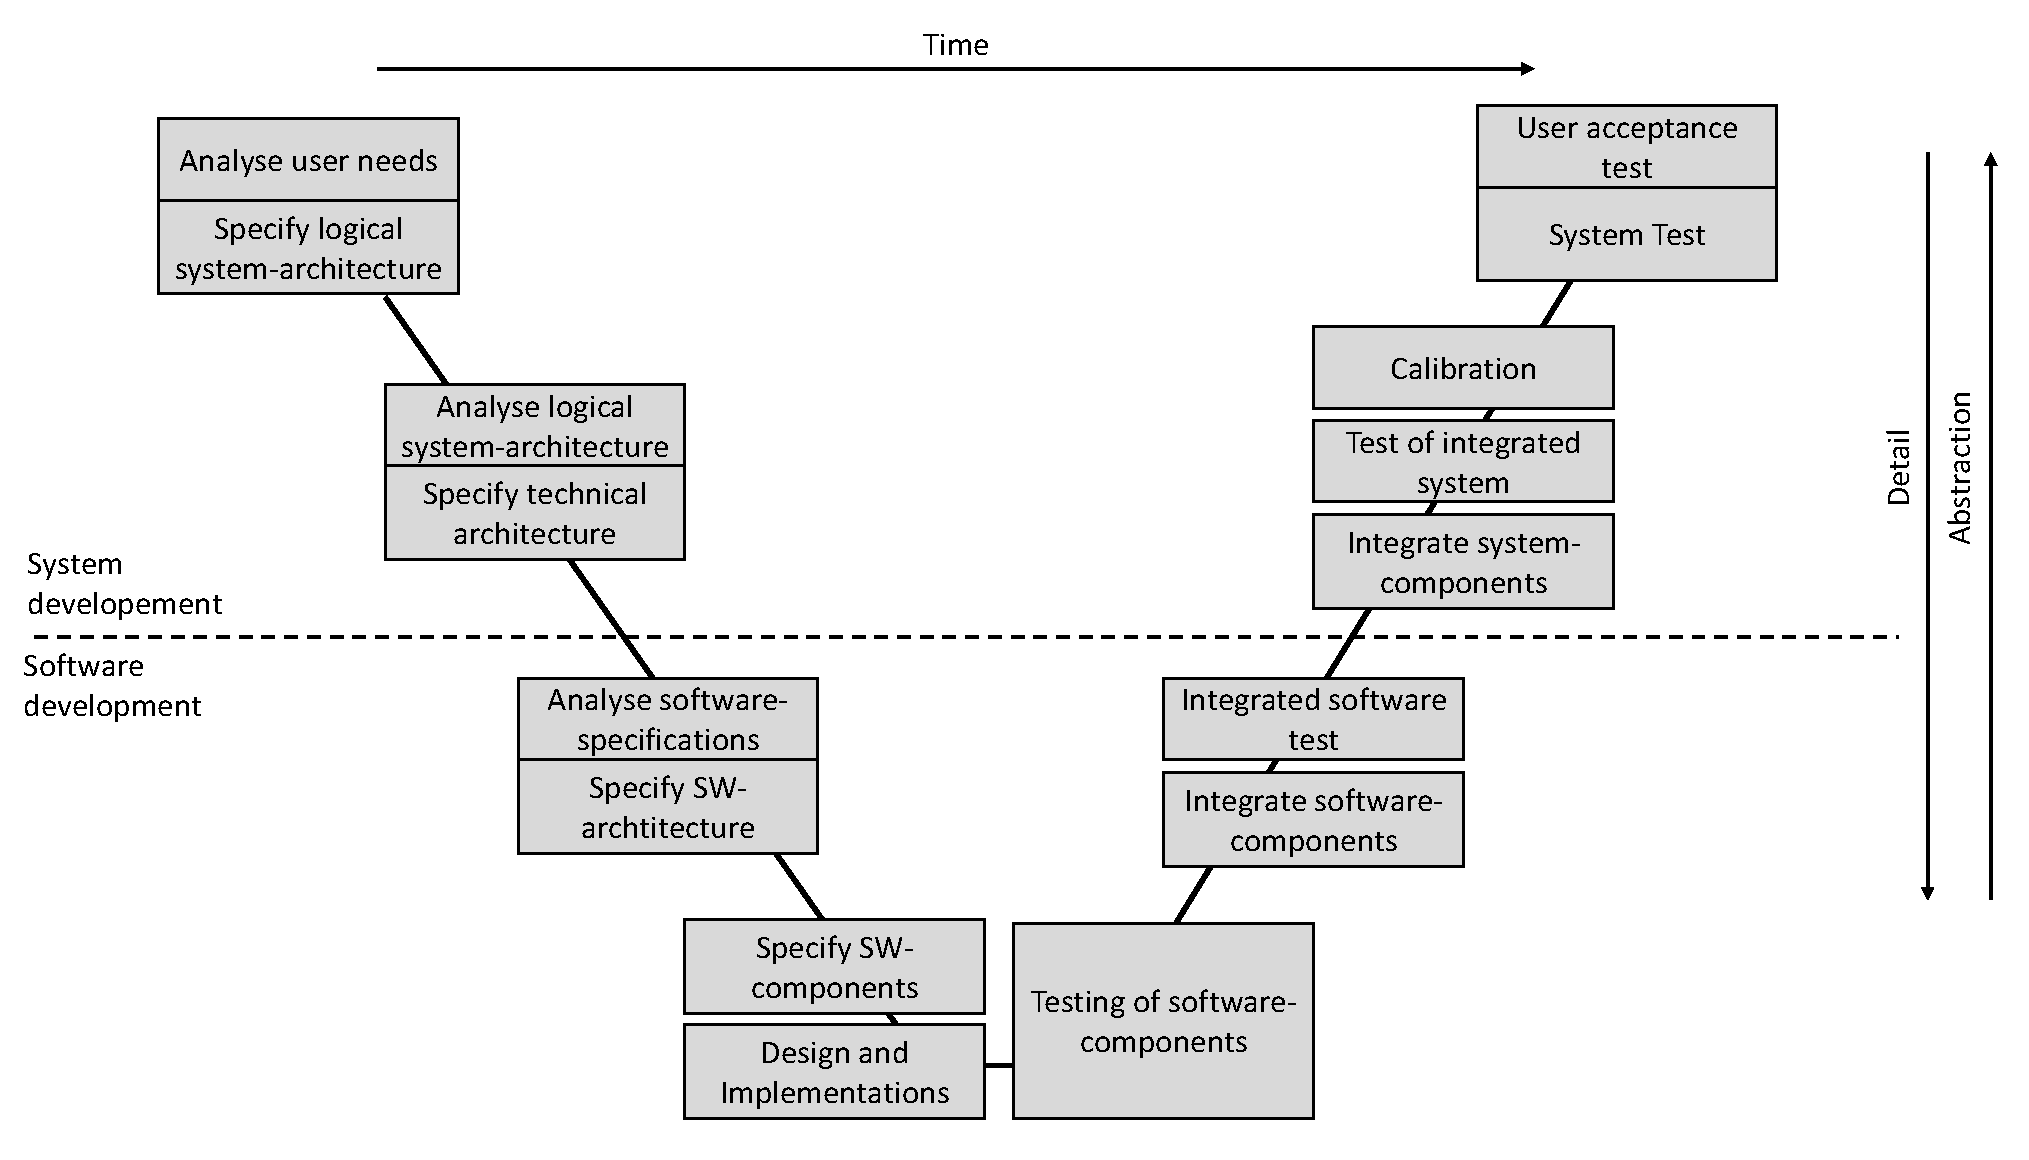
\includegraphics[width=0.9\linewidth]{figures/v_model/Folie1}
\caption{Overview for a process in automotive software development after the V-model}
\label{fig:v_model}
\end{figure*}



The increasing complexity of mechatronic systems and shorter product life-cycles lead to new development methods that made it possible to take 'short-cuts' in the established V-model process. This methods are summarized under the term rapid prototyping - in the case of software functions for mechatronic systems the term rapid control prototyping (RCP) was coined. It is possible to conduct testing and verification with early soft- and hardware versions which are still under development by having the remaining system and environmental influences simulated by the RCP-platform. In utilizing these new methods such as rapid control prototyping and software/hardware-in-the-loop testing, a tremendous decrease in development time can be achieved. It is also possible to validate specifications early in the process, eliminating possible cost-intensive changes in later stages.\cite{rapidcontrolprototyping} For the research project in which this theses is embedded it even opens up the possibility of on-road testing, as it eliminates the low-level development steps of the actual implementation and some of the detailed design work. The implementation of the steering algorithm (see section \ref{chap:steering_model}) on a stand-alone ECU, hydraulic actuator control, hardware layout, etc. would by far exceed the dimensions of a research project. Applying rapid control prototyping is the only feasible way to establish a functioning on-road prototype vessel.


\begin{itemize}
	\item V-model
	\item real-time capability
	\item abstract high level model to programm ==> focus on function development and modelling, no low level coding needed
	\item time critical processes
	\item extensive lecture notes from \cite{rapidcontrolprototyping}
\end{itemize}

\section{Overview of the model}
\label{sec:overview_of_the_model}
			
\begin{itemize}
	\item based on lit from MI-paper 
	\item overview graph of model
	\item single track model
	
	\item filtering of inputs?
	\item feedback-loop
	\item start condition
	\item what can be concluded with the model?
\end{itemize}

\section{Input parameters}
\label{sec:input_parameters}

\begin{itemize}
	\item what parameters are used as inputs? dimensions, min/max
	\item explain feedback/inverse path
	
\end{itemize}

\section{Real-Time implementation}
\label{sec:real_time_implementation}

\begin{itemize}
	\item what had to be changed to allow for MABII execution?
	\item how will feedback loop be handled?
	item incorporate measurings?
	\item simulation step size?
	\item utilized computational method
\end{itemize}

\section{Interface with Real-Time environment}
\label{sec:interface_with_real_time}

\begin{itemize}
	\item capabilities of system (see section \ref{sec:maxi_capabilities})
	\item signals passed forward from environment + restriction
	
	\item actuator signals
	\item signal modification (correct frequency for CAN)
	\item safety flags/signals
	
\end{itemize}

\end{document}
